% BHU PYQ -- Professional Exam Template
\documentclass[11pt,a4paper]{article}

\usepackage[a4paper,top=2.5cm,bottom=2.5cm,left=2.8cm,right=2.8cm,headheight=14pt]{geometry}
\usepackage{amsmath,amssymb}
\usepackage[T1]{fontenc}
\usepackage[utf8]{inputenc}
\usepackage{lmodern}
\usepackage{microtype}
\usepackage{fancyhdr}
\usepackage{enumitem}
\usepackage{hyperref}
\usepackage{lastpage}
\usepackage{parskip}
\usepackage{tikz}
\usetikzlibrary{arrows.meta,shapes,positioning}

\hypersetup{colorlinks=true,urlcolor=black,linkcolor=black,
  pdftitle={B.Sc. (Hons.) Zoology Sem-V ZOB-502 -- BHU PYQ}}

\pagestyle{fancy}
\fancyhf{}
\renewcommand{\headrulewidth}{0.4pt}
\renewcommand{\footrulewidth}{0.4pt}
\fancyhead[L]{\small   \textit{Banaras Hindu University}}
\fancyhead[R]{\small   \textit{Zoology Paper: ZOB-502}}
\fancyfoot[C]{\small Page  \thepage\ of \pageref{LastPage}}


\newlist{parts}{enumerate}{2}
\setlist[parts,1]{label=(\alph*),leftmargin=*,itemsep=4pt,topsep=3pt}
\setlist[parts,2]{label=(\roman*),leftmargin=*,itemsep=2pt,topsep=2pt}

\newcommand{\pts}[1]{\hfill   \textit{[#1]}}


\begin{document}


\begin{center}
  {\large\bfseries BANARAS HINDU UNIVERSITY}\\[2pt]
  {\normalsize B.Sc. (Hons.) Semester V Examination, 2022-23}\\[6pt]
  \rule{0.8\linewidth}{0.5pt}\\[6pt]
  {\large\bfseries Zoology}\\[4pt]
  {\large\bfseries Paper: ZOB-502 --- Functional Anatomy of Chordates}\\[4pt]
  {\normalsize Time: Three hours \hfill Full Marks: 70}
\end{center}

\rule{\linewidth}{0.4pt}

\smallskip



\noindent   \textit{Note: Answer six questions including Question No. 1 which is compulsory. The figures in the right-hand margin indicate marks.}

\bigskip




\noindent   \textbf{Question 1.} Answer the following parts:

\begin{parts}
  \item Answer whether the given statements are True or False with 2-3 lines justification:\pts{$5  \times 2 = 10$}
  
\begin{parts}
    \item Cycloid scales are derived from lamellar bone component.
    \item Crescent shaped cusps are characterised by Lophodont dentition.
    \item Opisthonephros is also called head kidney due to its anterior position.
    \item The oviduct is modified Wolffian duct in vertebrates.
    \item Mammalian lungs are structurally similar to avian lungs and have more efficient system of oxygen transport.
  \end{parts}
  
  \item Write in brief about the following:\pts{$5  \times 2 = 10$}
  
\begin{parts}
    \item Labyrinthodont teeth
    \item Antlers
    \item Archinephros
    \item Hepatic portal system
    \item Cerebral supremacy.
  \end{parts}
\end{parts}

\medskip


\noindent   \textbf{Question 2.} Illustrate the general features of integument in aquatic vertebrates. How does the organisation of the integument in these organisms (such as sharks) allow lateral bending of the body without distorting the body shape?\pts{10}

\medskip


\noindent   \textbf{Question 3.} With the help of a neat diagram, depict the different compartments of a ruminant stomach and their characteristics. Explain the mechanism behind the passage of food through these compartments.\pts{10}


\begin{center}

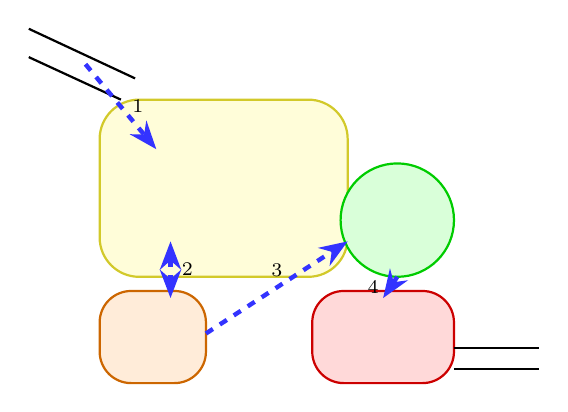
\begin{tikzpicture}[scale=0.9, >=Stealth, every node/.style={font=\small}]
  % Esophagus
  \draw[thick] (-3, 2.5) -- (-1.5, 1.8);
  \draw[thick] (-3, 2.1) -- (-1.7, 1.5);
  
ode[left] at (-3, 2.3) {Esophagus};
  
  % Rumen
  \draw[fill=yellow!15, draw=yellow!80!black, thick, rounded corners=0.5cm] (-2, -1) rectangle (1.5, 1.5);
  
ode at (-0.2, 0.2) {   \textbf{Rumen}};
  
  % Reticulum
  \draw[fill=orange!15, draw=orange!80!black, thick, rounded corners=0.4cm] (-2, -2.5) rectangle (-0.5, -1.2);
  
ode at (-1.25, -1.85) {   \textbf{Reticulum}};
  
  % Omasum
  \draw[fill=green!15, draw=green!80!black, thick, circle] (2.2, -0.2) circle (0.8);
  
ode at (2.2, -0.2) {   \textbf{Omasum}};
  
  % Abomasum
  \draw[fill=red!15, draw=red!80!black, thick, rounded corners=0.4cm] (1.0, -2.5) rectangle (3.0, -1.2);
  
ode at (2.0, -1.85) {   \textbf{Abomasum}};
  
  % Duodenum
  \draw[thick] (3.0, -2.0) -- (4.2, -2.0);
  \draw[thick] (3.0, -2.3) -- (4.2, -2.3);
  
ode[right] at (4.2, -2.15) {Duodenum};
  
  % Food flow arrows
  \draw[->, ultra thick, blue!80, dashed] (-2.2, 2.0) -- (-1.2, 0.8) node[midway, right, black, font=\scriptsize] {1};
  \draw[<->, ultra thick, blue!80, dashed] (-1.0, -0.5) -- (-1.0, -1.3) node[midway, right, black, font=\scriptsize] {2};
  \draw[->, ultra thick, blue!80, dashed] (-0.5, -1.8) -- (1.5, -0.5) node[midway, above, black, font=\scriptsize] {3};
  \draw[->, ultra thick, blue!80, dashed] (2.2, -1.0) -- (2.0, -1.3) node[midway, left, black, font=\scriptsize] {4};
\end{tikzpicture}
\end{center}

\pagebreak

\medskip


\noindent   \textbf{Question 4.} Describe the evolution of jaws in gnathostomes highlighting the suitable modifications in structure and their advantages.\pts{10}

\medskip


\noindent   \textbf{Question 5.} Write short notes on the following:\pts{$2  \times 5 = 10$}

\begin{parts}
  \item Lymph node
  \item Neuromast organ
\end{parts}

\medskip


\noindent   \textbf{Question 6.} Compare cross-current and counter-current mechanism of gaseous exchange with suitable examples and well-labelled diagram.\pts{10}


\begin{center}

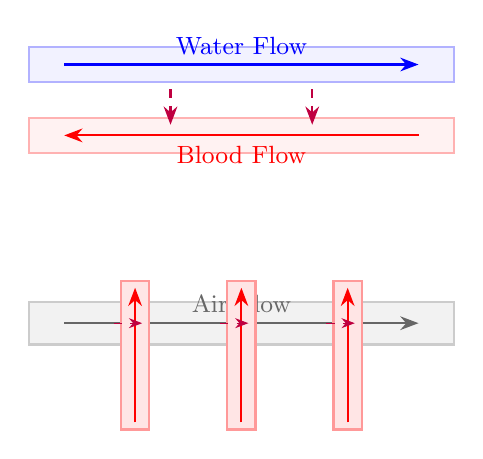
\begin{tikzpicture}[scale=0.9, >=Stealth, every node/.style={font=\small}]
  
\begin{scope}[shift={(0,0)}]
    
ode[above] at (3, 1.2) {   \textbf{A. Counter-Current Exchange (e.g., Fish Gills)}};
    % Water channel
    \draw[fill=blue!5, draw=blue!30, thick] (0,0.5) rectangle (6,1);
    \draw[->, thick, blue] (0.5, 0.75) -- (5.5, 0.75) node[midway, above] {Water Flow};
    
    % Blood channel
    \draw[fill=red!5, draw=red!30, thick] (0,-0.5) rectangle (6,0);
    \draw[<-, thick, red] (0.5, -0.25) -- (5.5, -0.25) node[midway, below] {Blood Flow};
    
    % Oxygen percentages
    
ode[font=\scriptsize] at (0.5, 0.75) {100\%};
    
ode[font=\scriptsize] at (2.0, 0.75) {70\%};
    
ode[font=\scriptsize] at (4.0, 0.75) {40\%};
    
ode[font=\scriptsize] at (5.5, 0.75) {15\%};
    
    
ode[font=\scriptsize] at (0.5, -0.25) {85\%};
    
ode[font=\scriptsize] at (2.0, -0.25) {60\%};
    
ode[font=\scriptsize] at (4.0, -0.25) {30\%};
    
ode[font=\scriptsize] at (5.5, -0.25) {5\%};
    
    % Diffusion
    \draw[->, thick, purple, dashed] (2, 0.4) -- (2, -0.1);
    \draw[->, thick, purple, dashed] (4, 0.4) -- (4, -0.1);
  \end{scope}

  
\begin{scope}[shift={(0,-3.2)}]
    
ode[above] at (3, 1.2) {   \textbf{B. Cross-Current Exchange (e.g., Avian Lungs)}};
    % Air capillary
    \draw[fill=gray!10, draw=gray!40, thick] (0,0) rectangle (6,0.6);
    \draw[->, thick, gray!80!black] (0.5, 0.3) -- (5.5, 0.3) node[midway, above] {Air Flow};
    
    % Blood capillaries
    \foreach \x in {1.5, 3.0, 4.5} {
      \draw[fill=red!10, draw=red!40, thick] (\x-0.2, -1.2) rectangle (\x+0.2, 0.9);
      \draw[->, thick, red] (\x, -1.1) -- (\x, 0.8);
      \draw[->, purple, dashed] (\x-0.3, 0.3) -- (\x+0.1, 0.3);
    }
  \end{scope}
\end{tikzpicture}
\end{center}

\medskip


\noindent   \textbf{Question 7.} What are aortic arches? How are they modified in Reptilia and Aves? Explain its evolutionary advantage in these classes.\pts{10}

\medskip


\noindent   \textbf{Question 8.} Name and describe the functional kidney found in amniotes. Describe the urinogenital system and their ducts in male and female vertebrates with well-labelled diagram.\pts{10}


\begin{center}

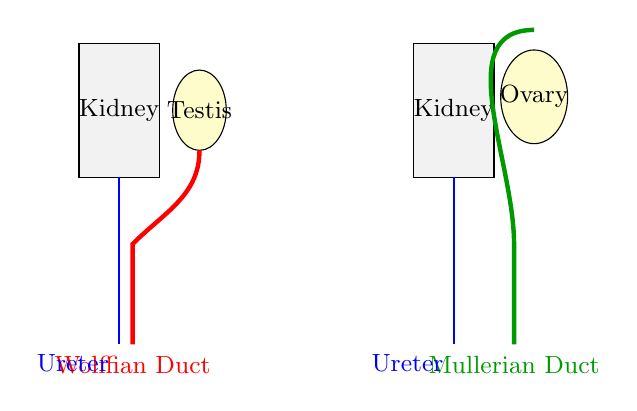
\begin{tikzpicture}[scale=0.85, >=Stealth, every node/.style={font=\small}]
  % Male
  
\begin{scope}[shift={(0,0)}]
    
ode[above] at (1, 3.5) {   \textbf{Male Vertebrate}};
    \draw[fill=gray!10, draw=black] (0, 1) rectangle (1.2, 3) node[pos=0.5] {Kidney};
    \draw[fill=yellow!20, draw=black] (1.8, 2) ellipse (0.4 and 0.6) node {Testis};
    
    \draw[ultra thick, red] (1.8, 1.4) to[out=-90, in=45] (0.8, 0) -- (0.8, -1.5) node[below] {Wolffian Duct};
    \draw[thick, blue] (0.6, 1.0) -- (0.6, -1.5) node[below left] {Ureter};
  \end{scope}
  
  % Female
  
\begin{scope}[shift={(5,0)}]
    
ode[above] at (1, 3.5) {   \textbf{Female Vertebrate}};
    \draw[fill=gray!10, draw=black] (0, 1) rectangle (1.2, 3) node[pos=0.5] {Kidney};
    \draw[fill=yellow!20, draw=black] (1.8, 2.2) ellipse (0.5 and 0.7) node {Ovary};
    
    \draw[ultra thick, green!60!black] (1.8, 3.2) to[out=180, in=90] (1.5, 0) -- (1.5, -1.5) node[below] {Mullerian Duct};
    \draw[thick, blue] (0.6, 1.0) -- (0.6, -1.5) node[below left] {Ureter};
  \end{scope}
\end{tikzpicture}
\end{center}

\vfill
\rule{\linewidth}{0.4pt}

\begin{center}\small
\href{https://bhu-exam.vercel.app/}{Click Here}\\[4pt]\href{https://me-aryan.vercel.app/}{Click Here}\\[4pt]\href{https://quashan-me.vercel.app/}{Click Here}
\end{center}

\end{document}
